\documentclass[tikz,margin=2mm]{standalone}
\pagestyle{empty}

%\usepackage{aistats2020}
\usepackage{amsmath}
\usepackage{bm}
\usetikzlibrary{positioning,calc,arrows,arrows.meta}

\begin{document}

	% PC algorithm MI test 400 samples
	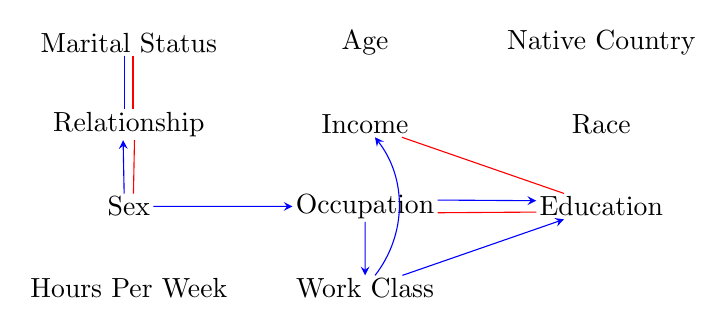
\begin{tikzpicture}
	\begin{scope}[xscale=1.2, yscale=1.3]
		\tikzstyle{every node}=[align=center, inner sep=1pt]
		\node (ms)   at (0, 0)    {{Marital Status}};
		\node (rln)  at (0, -0.8) {{Relationship}};
		\node (sex)  at (0, -1.6) {{Sex}};
		\node (hrpw) at (0, -2.4) {{Hours Per Week}};

		\node (age) at (2.5, 0)    {{Age}};
		\node (inc) at (2.5, -0.8) {{Income}};
		\node (occ) at (2.5, -1.6) {{Occupation}};
		\node (wc)  at (2.5, -2.4) {{Work Class}};

		\node (nc)   at (5, 0)    {{Native Country}};
		\node (race) at (5, -0.8) {{Race}};
		\node (edu)  at (5, -1.6) {{Education}};

		\draw [red, transform canvas={xshift=0.15em}] (ms) to (rln);
		\draw [blue, transform canvas={xshift=-0.15em} ] (ms) to (rln);

		\draw [red] (rln.-70) to (sex.70);
		\draw [red] (inc) to (edu);
		\draw [red] (occ.-5) to (edu.185);

		\draw [blue, ->, >=stealth] (sex.110) to (rln.-110);
		\draw [blue, ->, >=stealth] (sex) to (occ);
		\draw [blue, ->, >=stealth] (occ) to (wc);
		\draw [blue, ->, >=stealth] (occ.5) to (edu.175);
		\draw [blue, ->, >=stealth] (wc) to (edu);
		\draw [blue, ->, >=stealth] (wc) to[bend right=40] (inc);
	\end{scope}
	\end{tikzpicture}

	% PC algorithm Q3 test 400 samples
	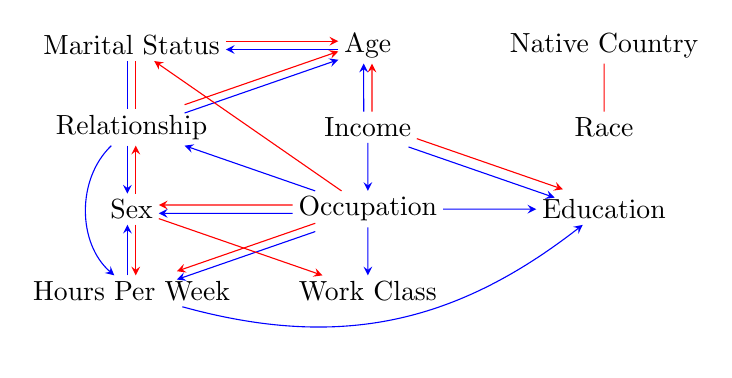
\begin{tikzpicture}
	\begin{scope}[xscale=1.2, yscale=1.3]
		\tikzstyle{every node}=[align=center, inner sep=0.2em]

		\node (ms)   at (0, 0)    {{Marital Status}};
		\node (rln)  at (0, -0.8) {{Relationship}};
		\node (sex)  at (0, -1.6) {{Sex}};
		\node (hrpw) at (0, -2.4) {{Hours Per Week}};

		\node (age) at (2.5, 0)    {{Age}};
		\node (inc) at (2.5, -0.8) {{Income}};
		\node (occ) at (2.5, -1.6) {{Occupation}};
		\node (wc)  at (2.5, -2.4) {{Work Class}};

		\node (nc)   at (5, 0)    {{Native Country}};
		\node (race) at (5, -0.8) {{Race}};
		\node (edu)  at (5, -1.6) {{Education}};


		\draw [red, transform canvas={xshift=0.15em}] (ms) to (rln);
		\draw [blue, transform canvas={xshift=-0.15em}] (ms) to (rln);

		\draw [red, ->, >=stealth, transform canvas={xshift=0.15em}] (sex) to (rln);
		\draw [blue,->, >=stealth, transform canvas={xshift=-0.15em}] (rln) to (sex);		

		\draw [red, ->, >=stealth, transform canvas={xshift=0.15em}] (sex) to (hrpw);
		\draw [blue,->, >=stealth, transform canvas={xshift=-0.15em}] (hrpw) to (sex);

		\draw [red, ->, >=stealth, transform canvas={yshift=0.15em}] (ms) to (age);
		\draw [blue,->, >=stealth, transform canvas={yshift=-0.15em}] (age) to (ms);

		\draw [red, ->, >=stealth, transform canvas={yshift=0.15em}] (rln) to (age);
		\draw [blue,->, >=stealth, transform canvas={yshift=-0.15em}] (rln) to (age);

		\draw [red, ->, >=stealth, transform canvas={xshift=0.15em}] (inc) to (age);
		\draw [blue,->, >=stealth, transform canvas={xshift=-0.15em}] (inc) to (age);
		\draw [red, ->, >=stealth, transform canvas={xshift=0.15em, yshift=0.15em}] (inc) to (edu);
		\draw [blue,->, >=stealth, transform canvas={xshift=-0.15em, yshift=-0.15em}] (inc) to (edu);

		\draw [red, ->, >=stealth, transform canvas={yshift=0.15em}] (occ) to (hrpw);
		\draw [blue,->, >=stealth, transform canvas={yshift=-0.15em}] (occ) to (hrpw);
		
		\draw [red, ->, >=stealth, transform canvas={yshift=0.15em}] (occ) to (sex);
		\draw [blue,->, >=stealth, transform canvas={yshift=-0.15em}] (occ) to (sex);
		
		
		\draw [red, ->, >=stealth] (sex) to (wc);
		\draw [red, ->, >=stealth] (occ) to (ms);
		\draw [red] (nc) to (race);

		\draw [blue,->, >=stealth] (rln) to[bend right=50] (hrpw);
		\draw [blue,->, >=stealth] (hrpw) to[bend right=25] (edu);
		
		\draw [blue,->, >=stealth] (inc) to (occ);
		\draw [blue,->, >=stealth] (occ) to (rln);
		\draw [blue,->, >=stealth] (occ) to (wc);
		\draw [blue,->, >=stealth] (occ) to (edu);

	\end{scope}
	\end{tikzpicture}

	% Hill Climb with BIC Score Q3 test 400 samples
	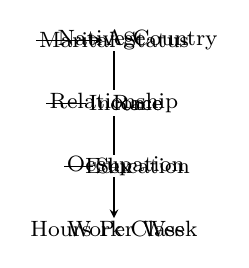
\begin{tikzpicture}
	\begin{scope}[xscale=0.1]
		\tikzstyle{every node}=[align=center, inner sep=1pt]

		\node (ms)   at (0, 0)    {\footnotesize{Marital Status}};
		\node (rln)  at (0, -0.8) {\footnotesize{Relationship}};
		\node (sex)  at (0, -1.6) {\footnotesize{Sex}};
		\node (hrpw) at (0, -2.4) {\footnotesize{Hours Per Week}};

		\node (age) at (1.5, 0)    {\footnotesize{Age}};
		\node (inc) at (1.5, -0.8) {\footnotesize{Income}};
		\node (occ) at (1.5, -1.6) {\footnotesize{Occupation}};
		\node (wc)  at (1.5, -2.4) {\footnotesize{Work Class}};

		\node (nc)   at (3, 0)    {\footnotesize{Native Country}};
		\node (race) at (3, -0.8) {\footnotesize{Race}};
		\node (edu)  at (3, -1.6) {\footnotesize{Education}};


		\draw [] (ms) to (rln);
		\draw [] (rln) to (sex);
		\draw [->, >=stealth] (sex) to (hrpw);

		\draw [->, >=stealth] (ms) to (age);
		\draw [] (rln) to (inc);
		\draw [] (sex) to (occ);
	\end{scope}
	\end{tikzpicture}

	% Hill Climb with BIC Score Q3 test 800 samples
	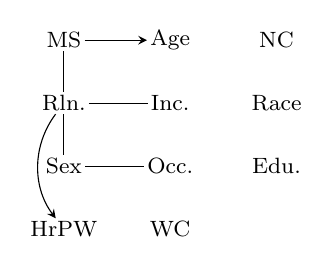
\begin{tikzpicture}
	\begin{scope}[xscale=0.9]
		\tikzstyle{every node}=[align=center, inner sep=1pt]

		\node (ms)   at (0, 0)    {\footnotesize{MS}};
		\node (rln)  at (0, -0.8) {\footnotesize{Rln.}};
		\node (sex)  at (0, -1.6) {\footnotesize{Sex}};
		\node (hrpw) at (0, -2.4) {\footnotesize{HrPW}};

		\node (age) at (1.5, 0)    {\footnotesize{Age}};
		\node (inc) at (1.5, -0.8) {\footnotesize{Inc.}};
		\node (occ) at (1.5, -1.6) {\footnotesize{Occ.}};
		\node (wc)  at (1.5, -2.4) {\footnotesize{WC}};

		\node (nc)   at (3, 0)    {\footnotesize{NC}};
		\node (race) at (3, -0.8) {\footnotesize{Race}};
		\node (edu)  at (3, -1.6) {\footnotesize{Edu.}};

		\draw [] (ms) to (rln);
		\draw [] (rln) to (sex);
		\draw [->, >=stealth] (rln) to[bend right=40] (hrpw);

		\draw [->, >=stealth] (ms) to (age);
		\draw [] (rln) to (inc);
		\draw [] (sex) to (occ);
	\end{scope}
	\end{tikzpicture}

\end{document}
